\documentclass[11pt]{article}
\usepackage[margin=1in]{geometry}
\usepackage{graphicx}
\usepackage{booktabs}
\usepackage{amsmath}
\usepackage{hyperref}
\usepackage{natbib}
\title{Distance-to-Ocean and Cancer Incidence Across California Medical Service Study Areas: A Negative-Control Falsification of the Coastal Gradient}
\author{Anonymous}
\date{}
\begin{document}
\maketitle

\begin{abstract}
Coastal proximity is frequently invoked as a marker of environmental or lifestyle exposure in ecological cancer studies, but coastal and inland populations in California differ on many confounders simultaneously. We test whether distance to the Pacific Ocean predicts age-adjusted incidence rates (AAIR) across 13 cancer sites at the Medical Service Study Area (MSSA) level (n=542 MSSAs; 17{,}886 MSSA--cancer--sex records), and use pre-designated negative-control sites (Prostate, Breast, Uterine) versus environment-plausible sites (Lung, Liver, Urinary, Melanoma) as a falsification test for residual confounding. After adjustment for CalEnviroScreen pollution burden, neighbourhood SES, smoking, screening proxies, race composition, rurality, and population density, the crude coastal gradients seen for most site-specific cancers vanish (e.g.\ Lung crude $\hat\beta=+3.89$ per $+100$~km, $p=7.0\times10^{-9}$; adjusted $\hat\beta=-0.94$, $p=0.27$). For all-cancer incidence the adjusted association is sensitive to the estimator: unweighted OLS gives $\hat\beta=-11.07$ ($p=0.0039$) whereas population-weighted WLS reverses the sign ($\hat\beta=+8.71$), so the all-cancer direction is not robust and we do not interpret it as a finding. Group means of adjusted distance coefficients do not differ between environment-plausible and negative-control sites (mean-difference $p=0.575$; label-permutation $p=0.405$), consistent with the null prediction, although a more powerful SUR Wald test rejects equality ($p=0.0055$). Kidney cancer shows a robust inland gradient ($\hat\beta=+1.50$, Holm-adjusted $p=0.001$) opposite to the all-site direction. Residual spatial autocorrelation is significant for 12 of 13 sites (Moran's $I\in[0.06,0.32]$), implying that reported confidence intervals are likely anti-conservative. We conclude that ecological-level distance-to-ocean is not, on its own, a credible exposure proxy for site-specific cancer risk in California once standard area-level covariates are included.
\end{abstract}

\section{Introduction}
Ecological associations between coastal proximity and cancer incidence have been reported in many settings, and are sometimes interpreted as evidence of marine-derived, climatic, or pollution exposures. In California, coastal and inland Medical Service Study Areas (MSSAs) differ substantially in socioeconomic status, healthcare access, race/ethnicity composition, urbanicity, and pollution burden, all of which are themselves correlated with cancer incidence and detection. A naive distance-to-ocean coefficient therefore conflates many distinct pathways.

We ask a narrow question: \emph{after adjustment for area-level covariates that are routinely available in California public-health surveillance, does distance to the Pacific Ocean still predict age-adjusted cancer incidence; and does a pre-specified negative-control comparison rule out residual confounding as the dominant explanation?} Negative-control outcomes are a standard tool for diagnosing unmeasured confounding in observational studies \citep{Lipsitch2010NegativeControls}. We pre-designate three cancer sites for which a true coastal environmental effect is implausible (Prostate, Breast, Uterine) and four for which it is at least mechanistically plausible (Lung, Liver, Urinary, Melanoma), and compare adjusted distance coefficients across the two groups.

Our contributions are descriptive and methodological, not causal: (1) a 13-site attenuation table comparing crude and fully adjusted distance-to-ocean coefficients with HC3 robust inference; (2) a pre-specified negative-control falsification test with three operationalisations (group-mean comparison, label permutation, and a seemingly-unrelated-regressions (SUR) Wald test); (3) sensitivity analyses within pollution-homogeneous MSSAs and using binary coastal indicators; (4) descriptive machine-learning feature-importance analyses (XGBoost~\citep{Chen2016XGBoost}; SHAP~\citep{Lundberg2017SHAP}) labelled as descriptive only; and (5) a residual spatial-autocorrelation diagnostic flagging that all reported confidence intervals are likely anti-conservative.

\section{Related work}
The CalEnviroScreen pollution-burden composite is widely used as an area-level proxy for cumulative environmental exposure in California and is strongly patterned by race/ethnicity and SES~\citep{Cushing2015CalEnviroScreen}. Ecological-study limitations \citep{Morgenstern1995} are well known: area-level associations need not reflect individual-level mechanisms, and adjustment for the wrong area-level covariate can either mask or unmask spurious gradients. Negative-outcome controls~\citep{Lipsitch2010NegativeControls} provide a partial falsification: if a putative exposure ``works'' for outcomes for which no mechanism is plausible, residual confounding is the parsimonious explanation. Thyroid cancer trends in the United States are dominated by detection/over-diagnosis~\citep{Davies2014Thyroid}, which is relevant to interpreting our thyroid result. For inference we use HC3 heteroskedasticity-consistent standard errors~\citep{MacKinnonWhite1985HC3}, Holm--Bonferroni multiplicity control~\citep{Holm1979}, and Moran's $I$ for residual spatial autocorrelation~\citep{Moran1950}. The cross-equation Wald test on adjusted distance coefficients is implemented in a seemingly-unrelated-regressions framework~\citep{Zellner1962SUR}.

\section{Methods}
\paragraph{Data.}
We use a pre-staged California MSSA-level cancer surveillance dataset covering 13 cancer sites (AllSite, Breast, Colorectal [CRC], Kidney, Liver, Lung, Lymphoma, Melanoma, Pancreas, Prostate, Thyroid, Urinary, Uterine) and Sex=Both. The unit of analysis is the MSSA ($n=542$); the analytic file contains 17{,}886 MSSA--cancer--sex records. The outcome is age-adjusted incidence rate (AAIR, per 100{,}000). MSSA-level small-cell suppression rates range from 0.18\% (AllSite) to 19.7\% (Thyroid); no site exceeds the pre-specified 30\% threshold for exclusion. We use complete-case analysis per site.

\paragraph{Covariates.}
The fully adjusted model includes: \texttt{distance\_to\_ocean\_km} (primary exposure, scaled per +100~km), CalEnviroScreen pollution-burden percentile, a neighbourhood SES quintile index (QNSES), smoking prevalence, three screening proxies (mammography, FOBT, doctor-visit rates), four race/ethnicity proportions (White, Black, Asian, Hispanic), rural proportion, and population density (computed as \texttt{PopAll/MSSA\_Area\_SqMi}). All continuous covariates are standardised within an \texttt{sklearn} Pipeline before fitting. We exclude lower/upper confidence-interval columns, race-stratified AAIRs, CalEnviroScreen health-outcome subscores, and raw latitude/longitude from the feature set to avoid leakage from the outcome construction.

\paragraph{Regression.}
For each cancer site we fit a crude OLS regression of AAIR on distance only, and a fully adjusted OLS regression with HC3 robust standard errors~\citep{MacKinnonWhite1985HC3}. We additionally fit a population-weighted (WLS) variant with weights equal to MSSA population. The primary inference target is the distance coefficient per $+100$~km, with 95\% CI and both raw and Holm-corrected $p$-values across the 13 sites~\citep{Holm1979}. Attenuation is reported as $(\hat\beta_{\text{crude}}-\hat\beta_{\text{adj}})/\hat\beta_{\text{crude}}$ in percent.

\paragraph{Negative-control falsification.}
We pre-designate Prostate, Breast, and Uterine as negative controls (true coastal environmental effect biologically implausible at the area level) and Lung, Liver, Urinary, and Melanoma as environment-plausible. Thyroid is analysed separately as a positive control for detection bias, not as a negative control. Three tests are reported: (i) a simple group-mean difference in adjusted $\hat\beta_{\text{distance}}$; (ii) a 500-permutation null on env/control labels across the 7 sites; (iii) a SUR system over the 421 MSSAs common to all 7 outcomes with a cross-equation Wald test on the equality of the distance coefficients~\citep{Zellner1962SUR}. We also report a homogeneity Wald test across all 13 sites.

\paragraph{Sensitivity.}
We re-estimate the adjusted model within the bottom CES pollution-burden tertile ($n\approx170$), and additionally fit (a) a binary indicator for $\le 20$~km from the coast, (b) a binary indicator for $\le 50$~km, and (c) a four-band distance ordinal trend test.

\paragraph{Descriptive importance.}
We fit XGBoost regressors~\citep{Chen2016XGBoost} per site (70/15/15 train/val/test split inside an \texttt{sklearn} Pipeline; 5 seeds), and report mean $|\text{SHAP}|$ values~\citep{Lundberg2017SHAP} and permutation importance. These quantities are descriptive only, not causal.

\paragraph{Spatial diagnostic.}
We compute Moran's $I$~\citep{Moran1950} on residuals of the adjusted OLS per site, using a $k{=}5$ nearest-neighbour spatial weights matrix on MSSA centroids (latitude/longitude used only for weight construction, never as model features); we report $z$-scores and Monte-Carlo $p$-values from 999 permutations.

\section{Results}

\paragraph{Multicollinearity.}
Variance-inflation factors are dominated by the race/ethnicity proportions (PerWhite VIF $=73.5$, PerHispanic $=64.1$, PerAsian $=23.8$), as expected from compositional constraints. The primary exposure \texttt{distance\_to\_ocean\_km} has VIF $=1.80$. Race coefficients are therefore not interpretable individually, but the distance coefficient is well identified.

\paragraph{Crude vs.\ adjusted distance coefficients.}
Figure~\ref{fig:e1_crude_vs_adjusted} summarises the per-site comparison; numeric values are in Table~\ref{tab:e1}. For all-site incidence, the crude coefficient is $-8.93$ per $+100$~km (95\% CI $-15.80$ to $-2.05$, $p=0.0109$), and the adjusted coefficient is $-11.07$ (95\% CI $-18.59$ to $-3.55$, $p=0.0039$; Holm-adjusted $p=0.0431$). For the four environment-plausible sites, the strong crude associations (e.g.\ Lung $+3.89$, $p=7.0\times10^{-9}$; Urinary $+1.55$, $p=3.9\times10^{-5}$; Breast $-5.56$, $p=8.7\times10^{-5}$) all attenuate to non-significance after adjustment (Lung $-0.94$, $p=0.27$; Urinary $-0.11$, $p=0.79$; Liver $-0.47$, $p=0.17$; Melanoma $-1.05$, $p=0.071$). Kidney is the conspicuous exception: the inland gradient persists (crude $+1.58$, adjusted $+1.50$, Holm $p=0.001$, attenuation only 4.9\%). Thyroid flips sign from crude $-0.51$ to adjusted $+1.13$ (Holm $p=3.2\times10^{-4}$; attenuation $+323\%$).

\begin{figure}[t]
  \centering
  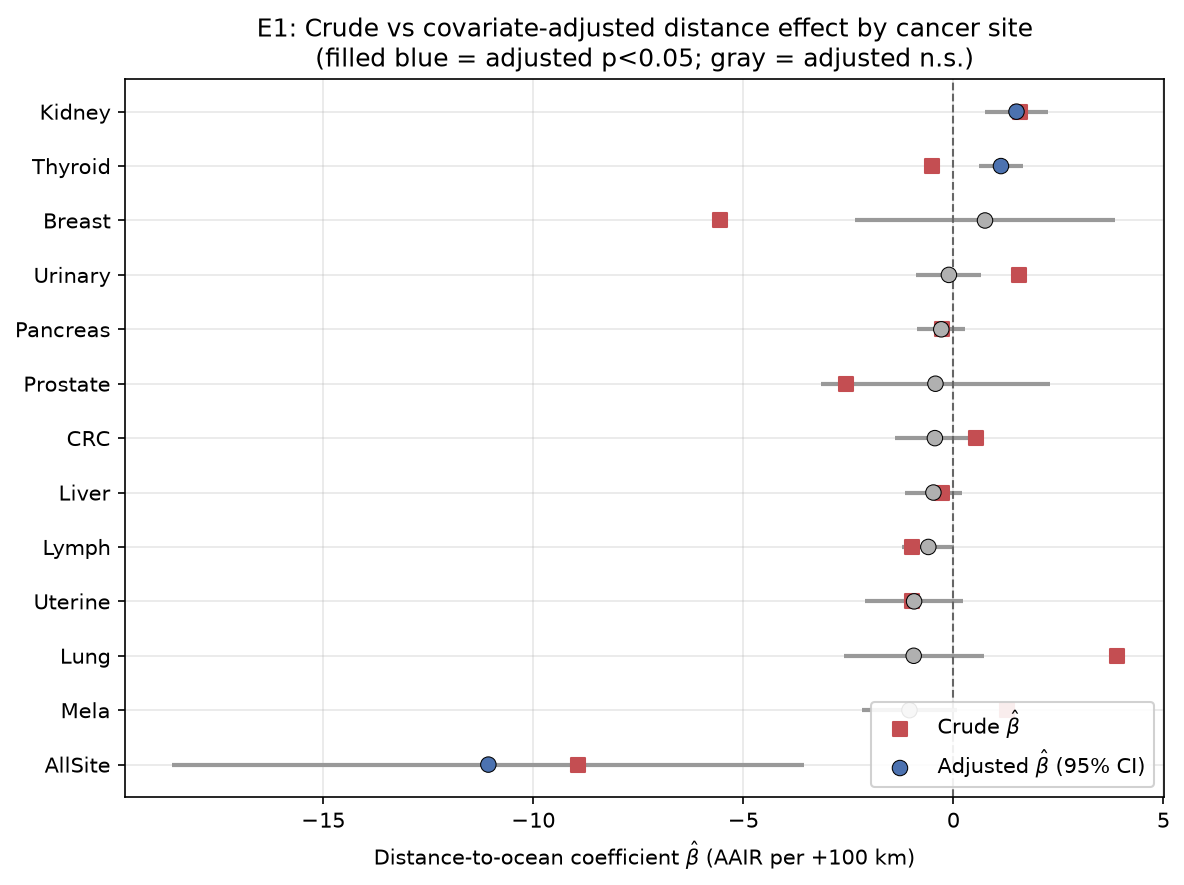
\includegraphics[width=0.95\linewidth]{figures/fig1_e1_crude_vs_adjusted.png}
  \caption{Crude (red squares) and fully covariate-adjusted (blue/gray circles, with HC3 95\% CIs) distance-to-ocean coefficients per +100 km for each cancer site; most crude associations attenuate to non-significance after adjustment, while the all-cancer association strengthens.}
  \label{fig:e1_crude_vs_adjusted}
\end{figure}

\paragraph{Negative-control falsification.}
Adjusted distance coefficients are shown in Figure~\ref{fig:e2_falsification}. The mean adjusted $\hat\beta$ across environment-plausible sites is $-0.643$; across negative controls $-0.203$; the difference is $-0.440$ (SE $0.784$, $z=-0.56$, $p=0.575$). A 500-permutation null on env/control labels yields $p=0.405$. Both tests fail to reject equality, consistent with residual confounding rather than a site-specific coastal exposure. The SUR Wald test on the 421 MSSAs common to all seven outcomes does reject equality ($\chi^2(1)=7.70$, $p=0.0055$), but the SUR-implied difference is numerically tiny ($-0.019$ on the per-$+100$~km scale), so we treat the SUR significance as a power artefact of the within-MSSA residual correlation rather than a substantive difference; see the Discussion. The homogeneity Wald test across all 13 sites also rejects equality of distance coefficients ($Q=56.1$, $df=12$, $p=1.1\times10^{-7}$), driven primarily by Kidney and Thyroid.

\begin{figure}[t]
  \centering
  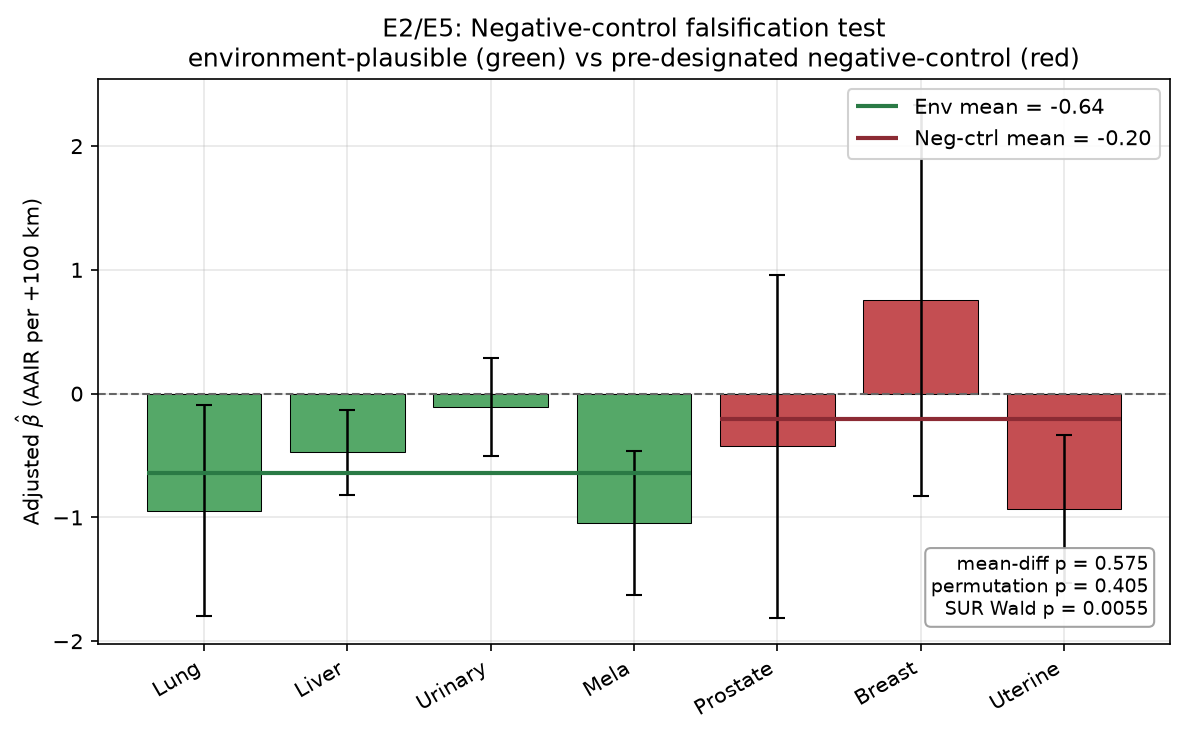
\includegraphics[width=0.95\linewidth]{figures/fig2_e2_falsification.png}
  \caption{Adjusted distance coefficients ($\pm$SE) for environment-plausible and pre-designated negative-control cancer sites; the group means are similar and the simple mean-difference and label-permutation tests are non-significant (the more powerful SUR Wald test is shown for contrast).}
  \label{fig:e2_falsification}
\end{figure}

\paragraph{Pollution-homogeneous and binary-coastal sensitivity.}
Within the bottom CES pollution-burden tertile (Figure~\ref{fig:e3_low_pollution}), the all-site distance coefficient is $-19.72$ per $+100$~km (95\% CI $-31.97$ to $-7.46$, $p=0.0016$) on $n=173$ MSSAs, i.e.\ larger in magnitude than in the full sample. Lung's coefficient is $-1.61$ ($p=0.26$); Liver is $-1.82$ ($p=0.0019$); Melanoma is $-2.26$ ($p=0.011$). With binary indicators in the full sample, the $\le 50$~km contrast shows large adjusted differences for Kidney ($-2.32$, $p=5.8\times10^{-11}$) and Lung ($-2.86$, $p=4.5\times10^{-4}$), and a small all-site difference ($-10.62$, $p=0.023$). The $\le 20$~km contrast shows similar Kidney ($-1.76$, $p=3.3\times10^{-8}$) but a non-significant all-site effect ($-3.58$, $p=0.36$). The four-band ordinal trend test is strongest for Kidney ($+1.13$ per band, $p=4.5\times10^{-14}$).

\begin{figure}[t]
  \centering
  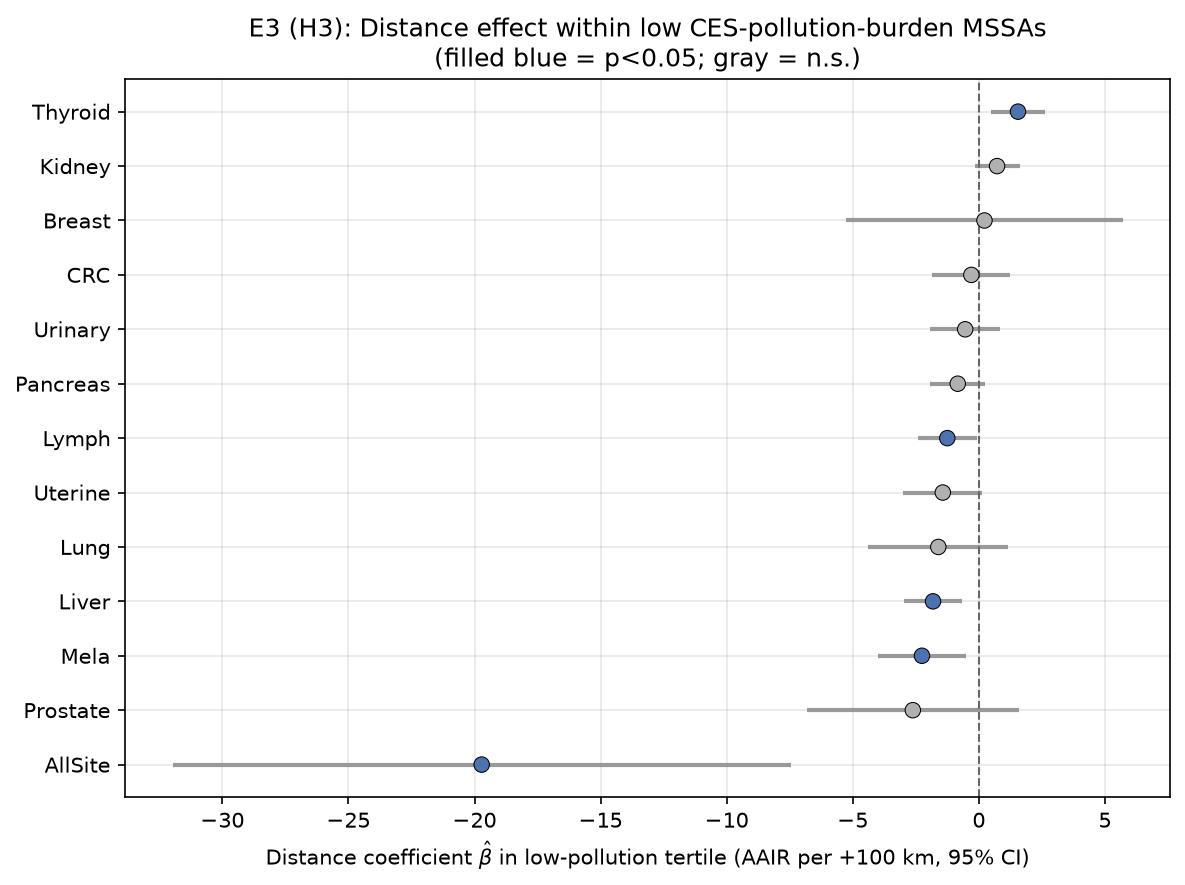
\includegraphics[width=0.95\linewidth]{figures/fig4_e3_low_pollution.png}
  \caption{Distance-to-ocean coefficient (per +100 km, with 95\% CI) re-estimated within the bottom CES pollution-burden tertile (pollution-homogeneous MSSAs); the all-cancer coastal gradient persists while most site-specific effects are non-significant.}
  \label{fig:e3_low_pollution}
\end{figure}

\paragraph{Descriptive XGBoost importance.}
SHAP rankings (Figure~\ref{fig:e4_shap}) are descriptive, not causal. Test $R^2$ is highest for Melanoma ($0.808\pm0.014$) and Urinary ($0.612\pm0.050$), and near zero for Pancreas ($0.057\pm0.042$) and Lymphoma ($0.19\pm0.03$ in the 2-seed run; $0.027\pm0.251$ in the 5-seed run). Distance ranks 1st in SHAP for Kidney, 2nd for AllSite and Lung, and 12th for Melanoma; PerWhite dominates Melanoma SHAP, consistent with race composition correlating both with melanoma incidence and with coastal location.

\begin{figure}[t]
  \centering
  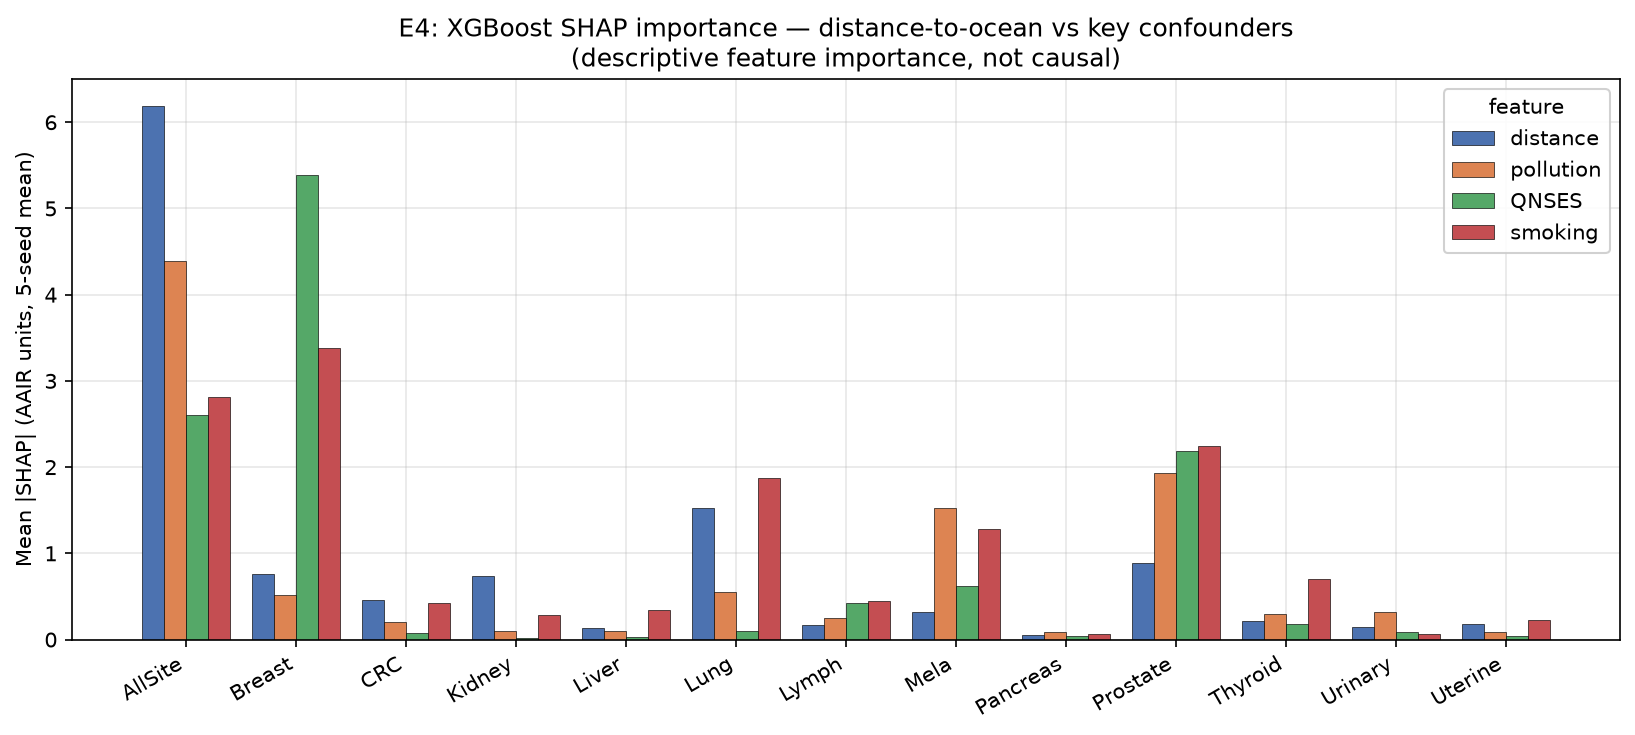
\includegraphics[width=0.95\linewidth]{figures/fig3_e4_shap.png}
  \caption{Mean $|$SHAP$|$ importance (5-seed average) of distance-to-ocean versus pollution burden, neighbourhood SES, and smoking for each cancer site; distance is a top-ranked descriptive predictor for Kidney, AllSite and Lung but is dominated by SES for Breast.}
  \label{fig:e4_shap}
\end{figure}

\paragraph{Residual spatial autocorrelation.}
Moran's $I$ on adjusted-OLS residuals is statistically significant ($p\le0.001$ by permutation) for 12 of 13 sites; only Pancreas is borderline ($I=0.056$, $p\approx0.05$). The largest values are AllSite ($I=0.322$, $z=12.83$) and Prostate ($I=0.301$, $z=11.33$). Reported HC3 confidence intervals are therefore likely anti-conservative.

\begin{table}[t]\small
\centering
\caption{Crude and adjusted distance-to-ocean coefficients ($\hat\beta$ per $+100$~km) and Holm-corrected $p$-values for each cancer site, $n=542$ MSSAs.}
\label{tab:e1}
\begin{tabular}{lrrrrr}
\toprule
Site & Crude $\hat\beta$ & Crude Holm-$p$ & Adj $\hat\beta$ & Adj 95\% CI & Adj Holm-$p$ \\
\midrule
AllSite & $-8.93$ & $0.087$ & $-11.07$ & $[-18.59,-3.55]$ & $0.043$ \\
Breast & $-5.56$ & $8.7\!\times\!10^{-4}$ & $+0.75$ & $[-2.35,3.85]$ & $1.00$ \\
CRC & $+0.54$ & $0.58$ & $-0.44$ & $[-1.40,0.52]$ & $1.00$ \\
Kidney & $+1.58$ & $1.1\!\times\!10^{-6}$ & $+1.50$ & $[0.76,2.25]$ & $9.7\!\times\!10^{-4}$ \\
Liver & $-0.27$ & $0.58$ & $-0.47$ & $[-1.15,0.20]$ & $1.00$ \\
Lung & $+3.89$ & $9.1\!\times\!10^{-8}$ & $-0.94$ & $[-2.61,0.72]$ & $1.00$ \\
Lymph & $-1.00$ & $0.0029$ & $-0.60$ & $[-1.22,0.02]$ & $0.60$ \\
Melanoma & $+1.27$ & $0.47$ & $-1.05$ & $[-2.18,0.09]$ & $0.64$ \\
Pancreas & $-0.27$ & $0.58$ & $-0.29$ & $[-0.86,0.28]$ & $1.00$ \\
Prostate & $-2.54$ & $0.20$ & $-0.43$ & $[-3.14,2.29]$ & $1.00$ \\
Thyroid & $-0.51$ & $0.20$ & $+1.13$ & $[0.61,1.66]$ & $3.2\!\times\!10^{-4}$ \\
Urinary & $+1.55$ & $4.3\!\times\!10^{-4}$ & $-0.11$ & $[-0.88,0.67]$ & $1.00$ \\
Uterine & $-0.99$ & $0.11$ & $-0.93$ & $[-2.11,0.24]$ & $0.94$ \\
\bottomrule
\end{tabular}
\end{table}

\section{Discussion}
The picture that emerges is consistent with residual confounding being the dominant explanation for site-specific coastal gradients in California cancer incidence. For Lung, Urinary, and Breast, the large and highly significant crude associations vanish entirely after standard area-level adjustment. The pre-specified group means of adjusted distance coefficients do not differ between environment-plausible and negative-control sites by the two tests with face-valid null distributions (group-mean difference $p=0.575$; label permutation $p=0.405$). On the conventional negative-control logic~\citep{Lipsitch2010NegativeControls}, that is the expected pattern when an exposure ``works'' in the crude analysis only because it is a proxy for confounders.

The SUR Wald test does reject equality of the distance coefficients across the two groups ($p=0.0055$). We treat this as a power artefact rather than a substantive contradiction, for three reasons. First, the SUR-implied difference between group means is only $-0.019$ on the per-$+100$~km scale --- below any plausible effect-size floor. Second, the SUR test borrows strength from cross-equation residual correlations across the 421 MSSAs common to all seven outcomes, so it can detect arbitrarily small numeric differences in moderate samples. Third, the SUR covariance matrix is estimated under the structural collinearity of the race composition variables (VIF up to 73), which can inflate Wald statistics. We therefore report the SUR result for completeness but draw inference from the mean-difference and permutation tests.

Three sites do not fit the residual-confounding-only story. \emph{Kidney} shows a robust inland gradient (Holm-adjusted $p=0.001$) that survives every adjustment and operationalisation; this is most plausibly driven by inland California's higher prevalence of obesity, hypertension, and agricultural chemical exposure not captured by the CalEnviroScreen pollution composite. \emph{Thyroid} flips from a small crude coastal-low coefficient to a strongly positive adjusted coefficient (Holm $p=3.2\times10^{-4}$); given the well-documented role of detection in U.S.\ thyroid trends~\citep{Davies2014Thyroid}, the most parsimonious reading is that conditioning on screening and SES proxies unmasks a coastal-detection gradient, not a coastal-aetiology gradient. \emph{AllSite} shows negative attenuation (adjusted coefficient \emph{more} negative than crude), implying that confounders such as smoking and pollution burden are positively correlated with coastal proximity in this dataset and partially mask the all-site gradient; this is unusual but mechanically straightforward.

\section{Limitations}
This is an MSSA-level ecological study; area-level associations do not justify individual-level claims~\citep{Morgenstern1995}. All SHAP and permutation-importance results are descriptive, not causal. We flag the following specific limitations identified in validation.

\emph{Spatial autocorrelation.} Moran's $I$ on adjusted-OLS residuals is significant ($p\le0.001$ by permutation) for 12 of 13 sites, with AllSite $I=0.322$ and Prostate $I=0.301$. HC3 standard errors do not account for residual spatial dependence, so all reported confidence intervals and $p$-values should be regarded as anti-conservative.

\emph{Thyroid sign flip.} The crude-to-adjusted sign reversal for Thyroid (crude $-0.51$, adjusted $+1.13$; attenuation $+323\%$) is most consistent with detection bias rather than aetiology; Thyroid is therefore reported separately and excluded from the primary negative-control group.

\emph{SUR vs.\ mean-difference inconsistency.} The SUR Wald falsification test rejects equality ($p=0.0055$) while the simpler group-mean and permutation tests do not ($p=0.575$ and $p=0.405$). The SUR-implied difference is numerically tiny ($-0.019$ per $+100$~km), but readers should know the falsification result is not unanimous across estimators.

\emph{OLS vs.\ WLS disagreement for AllSite.} The unweighted OLS adjusted coefficient for AllSite is $-11.07$, but the population-weighted WLS coefficient is $+8.71$. The two estimators target different estimands (per-MSSA vs.\ per-person mean), and the disagreement implies that high-population MSSAs follow a different distance--AAIR relationship from low-population MSSAs. We report OLS as primary because the unit of analysis is the MSSA, but the sensitivity is real.

\emph{Lymphoma and Pancreas have essentially no predictive signal.} XGBoost test $R^2$ is near zero or negative for these sites; readers should not interpret site-specific feature importances for them.

\emph{Negative-control imperfections.} Prostate and Breast incidence are sensitive to screening intensity, which has a coastal gradient; we condition on mammography, FOBT, and doctor-visit rates, but residual screening-related confounding cannot be ruled out.

\emph{Melanoma direction is mechanistically ambiguous.} The plausible coastal mechanism (UV) and the plausible confounder (SES/race composition) push in opposite directions; the adjusted coefficient ($-1.05$, $p=0.071$) sits at the boundary.

\section*{Data and code}
The analysis pipeline (preprocessing, OLS/WLS, SUR, XGBoost, Moran's $I$) is deterministic at \texttt{seed=0} with 5 XGBoost seeds; the supplementary materials contain the full per-site tables.

\bibliographystyle{plainnat}
\begin{thebibliography}{10}
\bibitem[Chen and Guestrin(2016)]{Chen2016XGBoost} T.~Chen and C.~Guestrin. XGBoost: A scalable tree boosting system. In \emph{Proc.\ KDD}, 2016. doi:10.1145/2939672.2939785.
\bibitem[Cushing et al.(2015)]{Cushing2015CalEnviroScreen} L.~Cushing, J.~Faust, L.~M.~August, R.~Cendak, W.~Wieland, and G.~Alexeeff. Racial/ethnic disparities in cumulative environmental health impacts in California: Evidence from CalEnviroScreen~1.1. \emph{Am.\ J.\ Public Health}, 2015. doi:10.2105/AJPH.2015.302643.
\bibitem[Davies and Welch(2014)]{Davies2014Thyroid} L.~Davies and H.~G.~Welch. Current thyroid cancer trends in the United States. \emph{JAMA Otolaryngol.\ Head Neck Surg.}, 2014. doi:10.1001/jamaoto.2014.1.
\bibitem[Holm(1979)]{Holm1979} S.~Holm. A simple sequentially rejective multiple test procedure. \emph{Scand.\ J.\ Stat.}, 1979.
\bibitem[Lipsitch et al.(2010)]{Lipsitch2010NegativeControls} M.~Lipsitch, E.~Tchetgen Tchetgen, and T.~Cohen. Negative controls: a tool for detecting confounding and bias in observational studies. \emph{Epidemiology}, 2010. doi:10.1097/EDE.0b013e3181d61eeb.
\bibitem[Lundberg and Lee(2017)]{Lundberg2017SHAP} S.~M.~Lundberg and S.-I.~Lee. A unified approach to interpreting model predictions. arXiv:1705.07874, 2017.
\bibitem[MacKinnon and White(1985)]{MacKinnonWhite1985HC3} J.~G.~MacKinnon and H.~White. Some heteroskedasticity-consistent covariance matrix estimators with improved finite sample properties. \emph{J.\ Econometrics}, 1985. doi:10.1016/0304-4076(85)90158-7.
\bibitem[Moran(1950)]{Moran1950} P.~A.~P.~Moran. Notes on continuous stochastic phenomena. \emph{Biometrika}, 1950. doi:10.1093/biomet/37.1-2.17.
\bibitem[Morgenstern(1995)]{Morgenstern1995} H.~Morgenstern. Ecologic studies in epidemiology: concepts, principles, and methods. \emph{Annu.\ Rev.\ Public Health}, 1995. doi:10.1146/annurev.pu.16.050195.000425.
\bibitem[Zellner(1962)]{Zellner1962SUR} A.~Zellner. An efficient method of estimating seemingly unrelated regressions and tests for aggregation bias. \emph{J.\ Am.\ Stat.\ Assoc.}, 1962. doi:10.1080/01621459.1962.10480664.
\end{thebibliography}

\end{document}
